\documentclass[letterpaper]{article}
\title{CS2323 Homework 4}
\author{CS18BTECH11001}
\usepackage{float}
\usepackage[legalpaper, lmargin=0.5in, rmargin=0.5in, tmargin=0.8in]{geometry}
\usepackage{amsmath}
\usepackage{amssymb}
\usepackage{graphicx}
\graphicspath{ {./images/} }
\renewcommand{\shapedefault}{\itdefault}
\begin{document}
\begin{large}
\maketitle
\begin{center}
\textit{This document is generated by \LaTeX}
\end{center}
\begin{flushleft}
\begin{enumerate}
\item[Q1. ]
The General formula for the time steps in which an array multiplication could be done using systolic array = $3n -2$.\\[0.1in]
\item[Q2. ]
for(rr=0; rr $<$ R;rr=rr+B)\\[0.1in]
for ( row=rr; row $<$ min(R,rr+B); row++)\\[0.1in]
for ( col =0; col $<$ C; col++)\\[0.1in]
for ( to=0; to $<$ M; to++)\\[0.1in]
for ( ti =0; ti $<$ N; ti++)\\[0.1in]
for ( i =0; i $<$ K; i++)\\[0.1in]
for ( j =0; j $<$ K; j++)\\[0.1in]
Output\_fmaps[to][row][col] += Weights[to][ti][i][j] $\times$ Input\_fmaps[ti][S$\times$row+i][S$\times$col+j]\\[0.1in]

\item[Q3. ]
\_device\_ void addFunc1(int *a, int *b, int *c)\\[0.1in]
\_global\_ void addFunc2(int *a, int *b, int *c)\\[0.1in]
\_host\_ void random\_ints(int* x, int size)\\[0.1in] 
\_host\_ int main(void)\\[0.1in]
\item[Q4. ]
Location of array/variables to be stored\\
\begin{table}[h]
\centering
\begin{tabular}{|c|c|}
\hline
Variables & Location\\
\hline
x\_ dim & local(register)\\
\hline
y\_ dim & local(register)\\
\hline
iteration & local(register)\\
\hline
pqr & local memory \\
\hline
ABC & global memory\\
\hline
maxValue & global memory\\
\hline
\end{tabular}
\end{table}
\item[Q5. ]
\begin{enumerate}
\item[a) ]
The dimension of matrix = 16$\times$16\\[0.1in]
Cache Size=128B\\[0.1in]
\item[b) ]
\underline{Unblocked Cache :}\\[0.1in]
Total hits for unblocked cache = 192\\[0.1in]
Total misses for unblocked cache = 320\\[0.1in]
Misses coming from input matrix=64\\[0.1in]
Misses coming from output matrix=256\\[0.1in]
\underline{Blocked Cache :}\\[0.1in]
Total hits for blocked cache = 384\\[0.1in]
Total misses for blocked cache = 128\\[0.1in]
Misses coming from input matrix=64\\[0.1in]
Misses coming from output matrix=64\\[0.1in]
\end{enumerate}
\item[Q6. ]
Snapshot from T=0 to T=4 :\\[0.1in]
T=0:
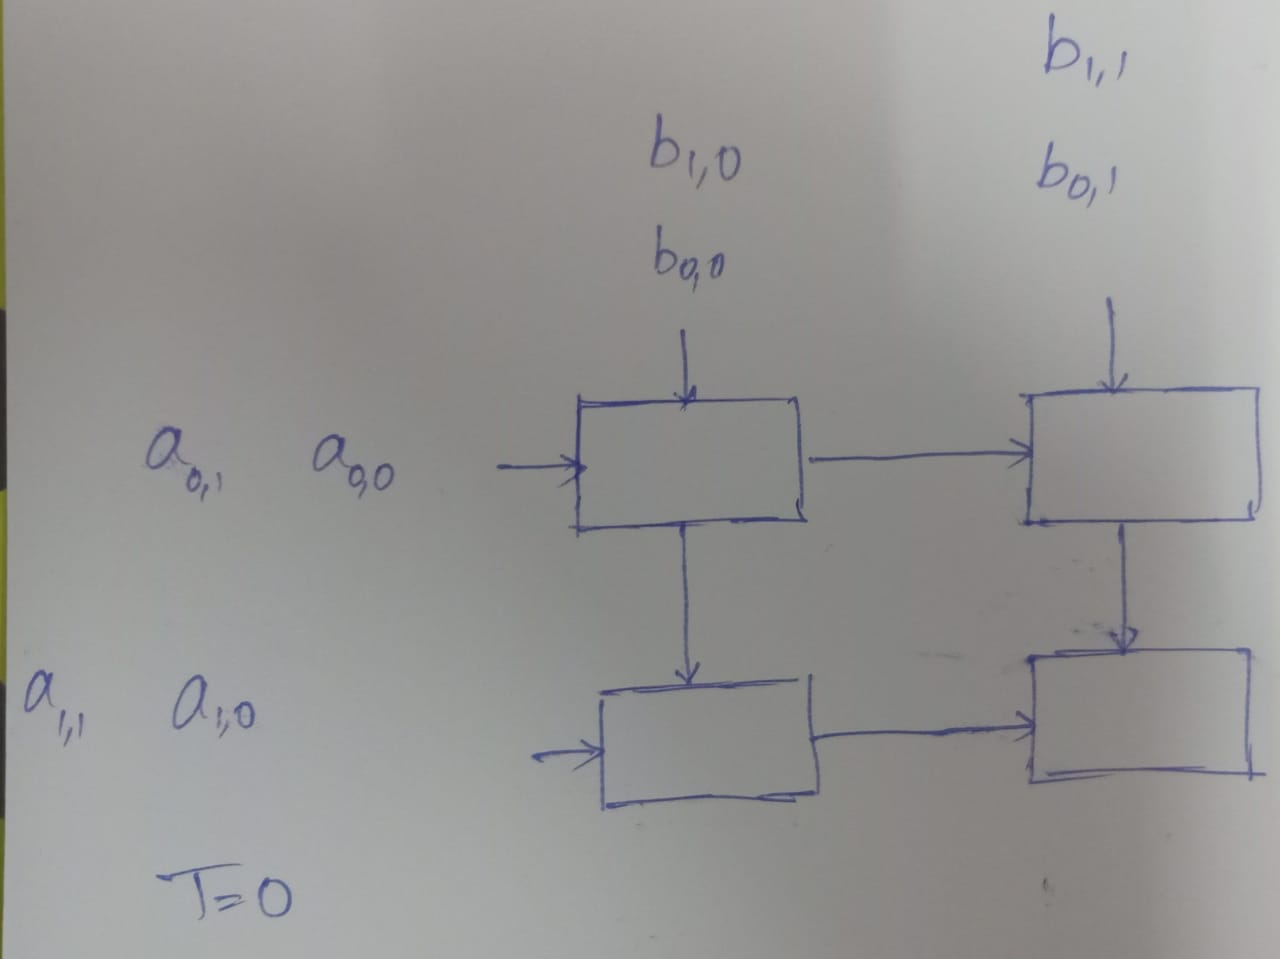
\includegraphics[width = 15cm,height = 5cm]{T=0}\\[0.1in]
T=1:
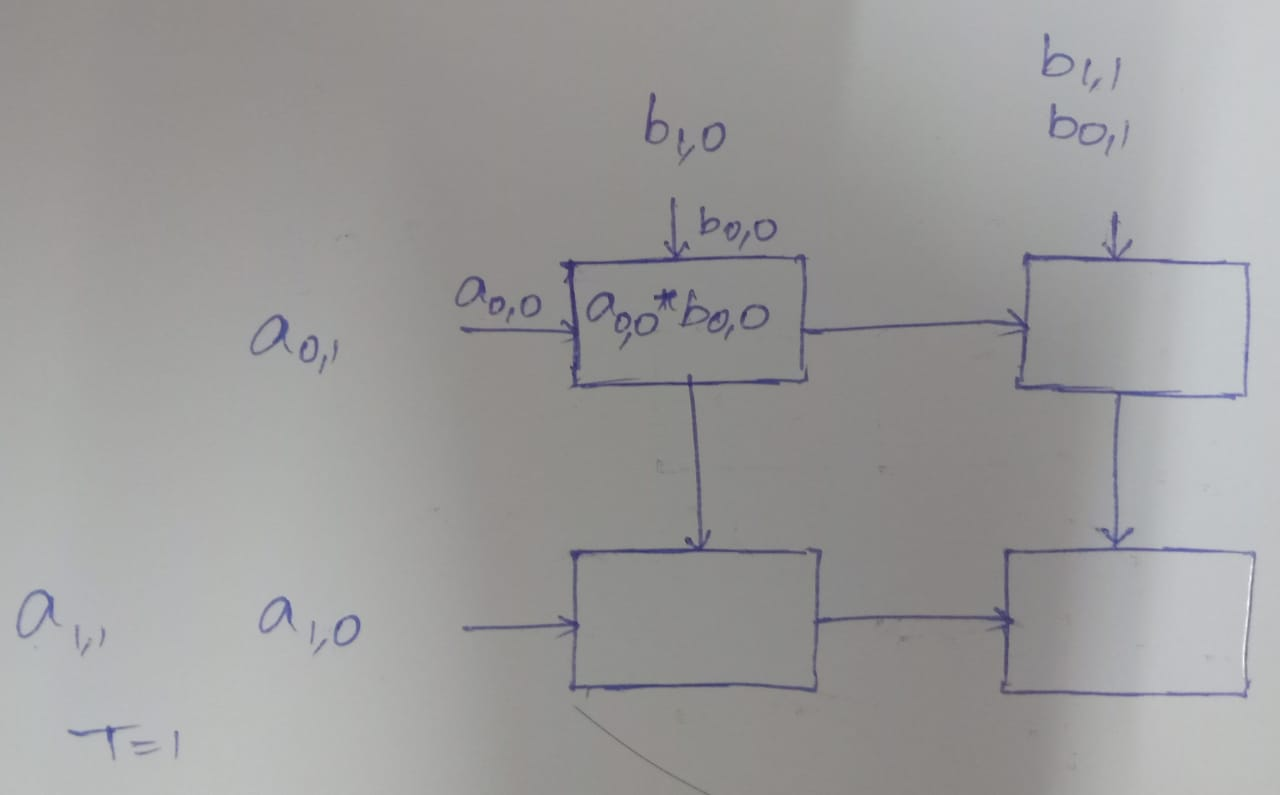
\includegraphics[width = 15cm,height = 5cm]{T=1}\\[0.1in]
T=2:
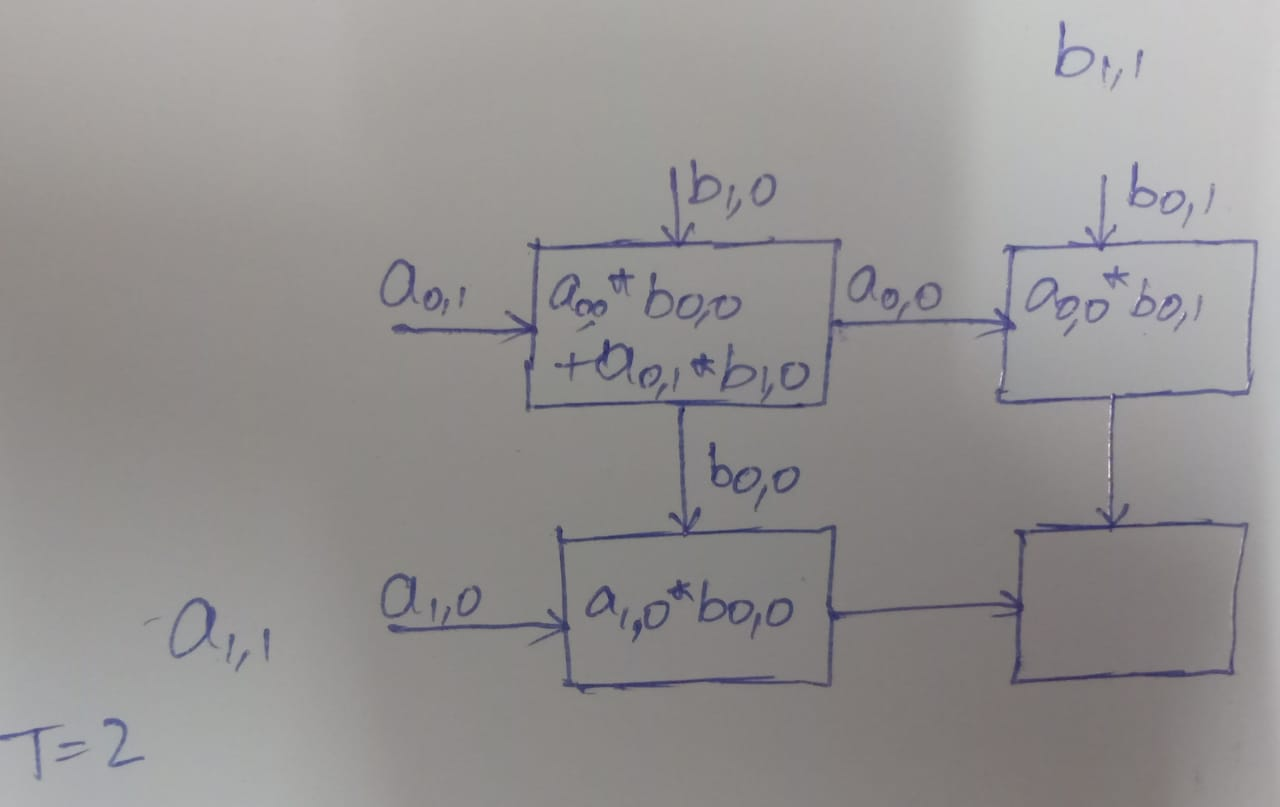
\includegraphics[width = 15cm,height = 5cm]{T=2}\\[0.1in]
T=3:
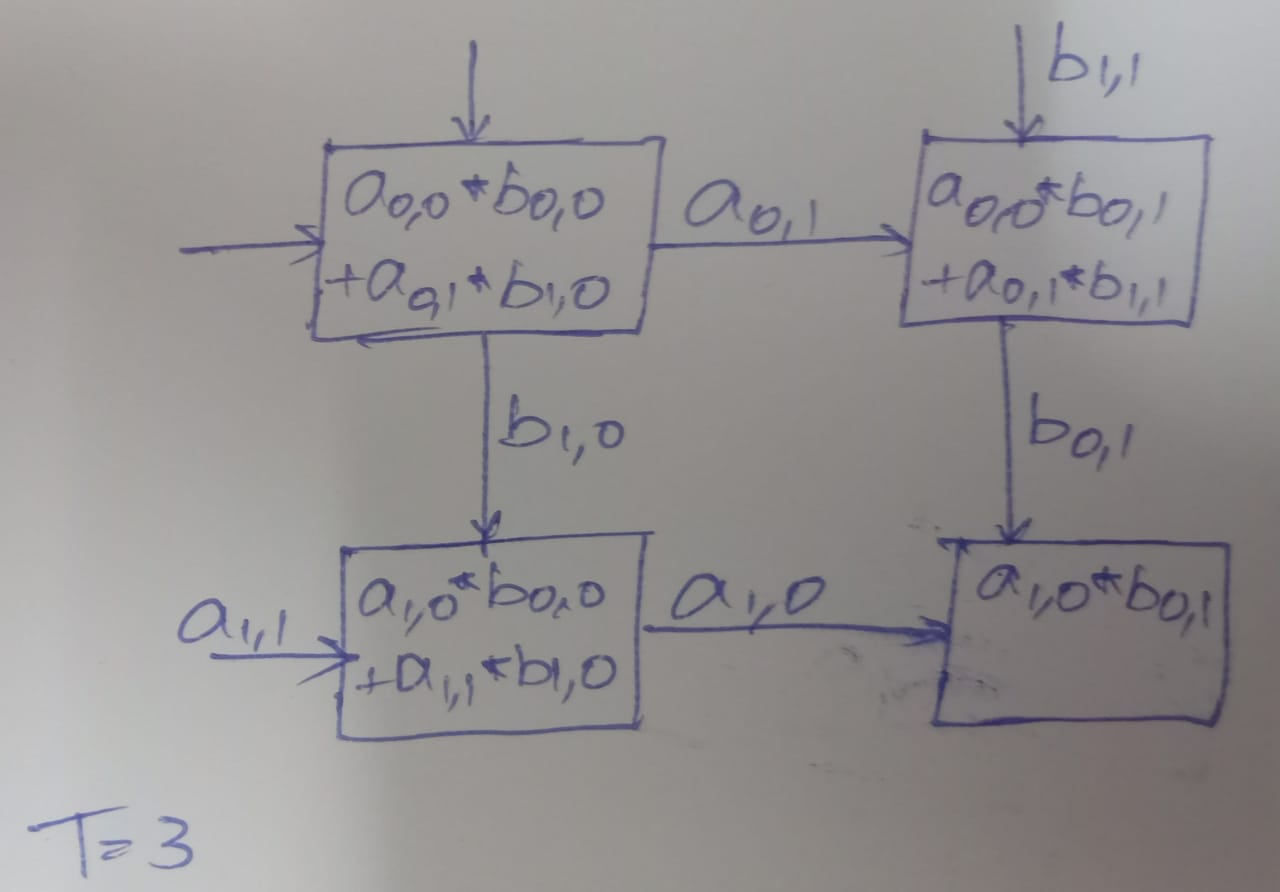
\includegraphics[width = 15cm,height = 5cm]{T=3}\\[0.1in]
T=4:
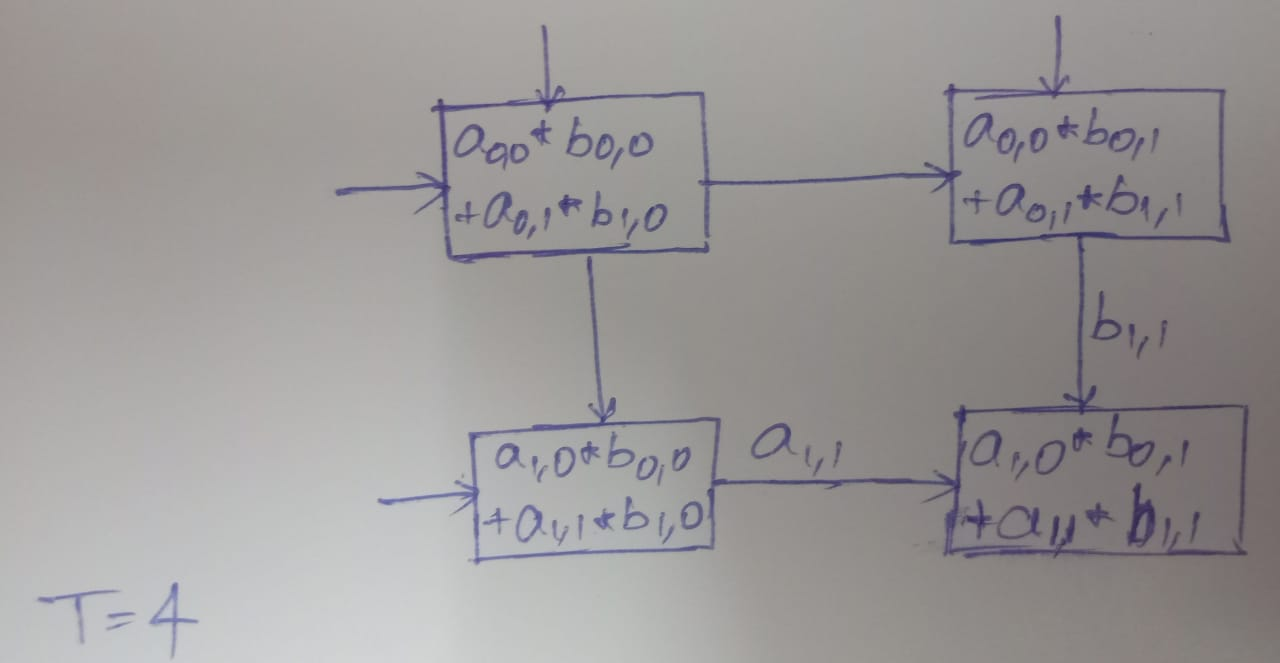
\includegraphics[width = 15cm,height = 5cm]{T=4}\\[0.1in]
\clearpage
\item[Q7. ]
\begin{enumerate}
\item[a) ]4
\item[b) ]5.5
\item[c) ]5.6875
\item[d) ]5.6953125
\end{enumerate}
\item[Q8. ]
Instruction : v.ld vr1,20[r2]\\[0.1in]
Semantics : vr1 $\leftarrow$ ([r2+20],[r2+24])\\[0.1in]
\item[Q9. ]
\begin{enumerate}
\item[a) ]
AI for case 1 = $\dfrac{Total\ no.\ of\ fp\ operations}{Total\ DRAM\ bytes}=\dfrac{N^2}{N^2*3*8}=1/24$\\[0.1in]
AI for case 2 = $\dfrac{Total\ no.\ of\ fp\ operations}{Total\ DRAM\ bytes}=\dfrac{N^2/4}{N^2*3*8}=1/96$\\[0.1in]
\item[b) ]
AI for case 1 = $\dfrac{Total\ no.\ of\ fp\ operations}{Total\ DRAM\ bytes}=\dfrac{N^2}{N^2*3*8}=1/24$\\[0.1in]
AI for case 2 = $\dfrac{Total\ no.\ of\ fp\ operations}{Total\ DRAM\ bytes}=\dfrac{N^2/4}{\dfrac{N^2}{4}*3*8}=1/24$\\[0.1in]
\end{enumerate}
\item[Q10. ]
\begin{enumerate}
\item[a) ]
No. of GOPS required to classify 1 image = 1.5\\[0.1in]
No. of GOPS available at peak performance = 0.75$\times$66$\times$1000=49500\\[0.1in]
No. of images that can be classified = $\dfrac{49500}{1.5}$ = 33000\\[0.1in]
\item[b) ]
AI for 8b fixed point versions = $\dfrac{1.5\times 10^{9}}{50 \times 1024 \times 1024 \times 1024}=28.61022\ operations/B$\\[0.1in]
AI for binarized versions = $\dfrac{1.5\times 10^{9}}{7.4 \times 1024 \times 1024 \times 1024}=193.31236\ operations/B$\\[0.1in]
\end{enumerate}
\item[Q11. ]
Arithmetic intensity required for achieving peak FLOP on using MCDRAM = $\dfrac{2199}{372}=5.91129$\\[0.1in]
arithmetic intensity required for achieving peak FLOP on using DRAM = $\dfrac{2199}{77}=28.55844$\\[0.1in]
\end{enumerate}
\end{flushleft}
\end{large}
\end{document}